\documentclass[onecolumn, draftclsnofoot,10pt, compsoc]{IEEEtran}
\usepackage{url}
\usepackage{setspace}
\usepackage{graphicx}
\usepackage{epstopdf}
\epstopdfsetup{update} % only regenerate pdf files when eps file is newer
\usepackage[utf8]{inputenc}
\usepackage[english]{babel}
\usepackage{indentfirst}
\usepackage{geometry}
\usepackage{color}
\usepackage{tikz}
\usepackage{rotating}
\usepackage{pgfgantt}
\usepackage{xcolor}
\geometry{textheight=9.5in, textwidth=7in}


\newganttchartelement{orangebar}{
    orangebar/.style={
        inner sep=0pt,
        draw=red!66!black,
        very thick,
        top color=white,
        bottom color=orange!80
    },
    orangebar label font=\slshape,
    orangebar left shift=.1,
    orangebar right shift=-.1
}

\newganttchartelement{bluebar}{
    bluebar/.style={
        inner sep=0pt,
        draw=purple!44!black,
        very thick,
        top color=white,
        bottom color=blue!80
    },
    bluebar label font=\slshape,
    bluebar left shift=.1,
    bluebar right shift=-.1
}


% 1. Fill in these details
\def \CapstoneTeamName{		MAV Challenge}
\def \CapstoneTeamNumber{		32}
\def \GroupMemberOne{			Justin Sherburne}
\def \GroupMemberTwo{			Kaiyuan Fan}
\def \GroupMemberThree{			Yingshi Huang}
\def \CapstoneProjectName{		AHS Micro-Air Vehicle Challenge}
%\def \CapstoneSponsorCompany{	Columbia Helicopters}
\def \CapstoneSponsorPerson{		Nancy Squires, Ph.D.}

% 2. Uncomment the appropriate line below so that the document type works
\def \DocType{		%Problem Statement
				%Requirements Document
				%Technology Review
				Design Document
				%Progress Report
				}
			
\newcommand{\NameSigPair}[1]{\par
\makebox[2.75in][r]{#1} \hfil 	\makebox[3.25in]{\makebox[2.25in]{\hrulefill} \hfill		\makebox[.75in]{\hrulefill}}
\par\vspace{-12pt} \textit{\tiny\noindent
\makebox[2.75in]{} \hfil		\makebox[3.25in]{\makebox[2.25in][r]{Signature} \hfill	\makebox[.75in][r]{Date}}}}
% 3. If the document is not to be signed, uncomment the RENEWcommand below
\renewcommand{\NameSigPair}[1]{#1}

%%%%%%%%%%%%%%%%%%%%%%%%%%%%%%%%%%%%%%%
\begin{document}
\begin{titlepage}
    \pagenumbering{gobble}
    \begin{singlespace}
    	
\includegraphics[height=4cm]{coe_v_spot1}
        \hfill 
        % 4. If you have a logo, use this includegraphics command to put it on the coversheet.
        %\includegraphics[height=4cm]{CompanyLogo}   
        \par\vspace{.2in}
        \centering
        \scshape{
            \huge CS Capstone \DocType \par
            {\large\today}\par
            \vspace{8pt}
            \textbf{\Huge\CapstoneProjectName}\par
			\vspace{1.5in}
            {\large Prepared for}\par
            % \Huge \CapstoneSponsorCompany\par
            % \vspace{5pt}
            {\Large\NameSigPair{\CapstoneSponsorPerson}\par}
			\vspace{3pt}
            {\large Prepared by }\par
            Group\CapstoneTeamNumber\par
            % 5. comment out the line below this one if you do not wish to name your team
            \CapstoneTeamName\par 
            \vspace{8pt}
            {\Large
                \NameSigPair{\GroupMemberOne}\par
                \NameSigPair{\GroupMemberTwo}\par
                \NameSigPair{\GroupMemberThree}\par
            }
            \vspace{.5in}
        }
        \begin{abstract}
        The purpose of this document is to elaborate on design concepts related to the implementation of the Micro Air Vehicle project. Our goal is to provide our intended audience with information on the design and implementation of our core features. Here we will outline technical concerns and viewpoints contained within the scope of the Micro Air Vehicle project. 
        \end{abstract}     
    \end{singlespace}
\end{titlepage}
\newpage
\pagenumbering{arabic}
\tableofcontents
% 7. uncomment this (if applicable). Consider adding a page break.
\listoffigures
%\listoftables
\clearpage


\section*{Revision History}

\begin{center}
    \begin{tabular}{|c|c|c|c|}
        \hline
		Name & Date & Reason For Changes & Version\\
        \hline
		Design Document & Nov 29, 2017 & Initial Creation & 1.0\\
		\hline 
    \end{tabular}
\end{center}




\section{Overview}


\subsection{Scope}% of the document

This document is intended to inform the reader of the technical goals of the Micro Air Vehicle Challenge project. Here we will describe subcomponents of the project, and how each subcomponent will be implemented into the overall design. It will provide a clear framework for each piece, and provide viewpoints on how each element will be designed. It is not a definition of requirements, or a concrete timeline of events leading up to the completion of the project.


\subsection{Purpose}% of the document

The purpose of this document is to describe how our project will be implemented to accomplish the tasks defined by the AHS 6th annual MAV challenge. The goal of this project is to create a remotely piloted helicopter with an autonomous flight feature. This document will explain the details of the project's design.


\subsection{Intended Audience}

The intended audience of this design document is project team members, project sponsors or facilitators, and project collaborators.  

\section{Definitions} % Alphabetized?
\begin{description}
		\item{AHS} -  American Helicopter Society.
        \item{Autonomous} -  Acting independently from any controlling source.
        \item{CSI} - Camera Serial Interface. This is the primary interface for the Raspberry Pi cameras. 
        \item{ESC} - Electronic Speed Controller. Used to control motor speed with low voltage logic. 
        \item{GUI} -  Graphical User Interface.
        \item{GPIO} - General-purpose input/output.
        \item{MAV} -  Micro Air Vehicle.
        \item{USB} - Universal Serial Bus
        
\end{description}     


\section{System requirements} 


\subsection{Functional Requirements}  

\begin{itemize}
\item The vehicle must weigh less than 500 grams including the battery.
\item The vehicle must be shorter than 17.7 inches in any one dimension. 
\item The vehicle is required to operate from an electric power source.
\item It must be able to take off and land vertically, and have the ability to maintain a stable altitude (hover).
\item It must have some sort of on-board camera system featuring at least one camera.
\item It must use standard communication methods, with a preference on 2.4GHz communications.
\item It must have an emergency cutoff switch that will power off the vehicles motors in case of a loss of communication.
\item It must have a manual control override so an operator can steer the vehicle back to the competition area. 
\end{itemize}


\subsection{Non-functional Requirements} 

\begin{itemize}
\item{The vehicle should be able to navigate the competition area without human intervention.}
\item{The cameras should maintain a minimum quality of 540p at 30fps.}
\item{The image progessing system should recognize each of the following objects: landing areas, packages, boundary lines, and large obstacles.}
\item{Hardware should be light enough and small enough to fit within the vehicle limitations.}
\item{WiFi communication should maintain a steady connection at a distance of more than 50 ft. }
\end{itemize}



\section{Conceptual Designs}%  for the project


\subsection{Design Overview} %Concept sketch + brief description

\begin{figure}[ht]
\centering
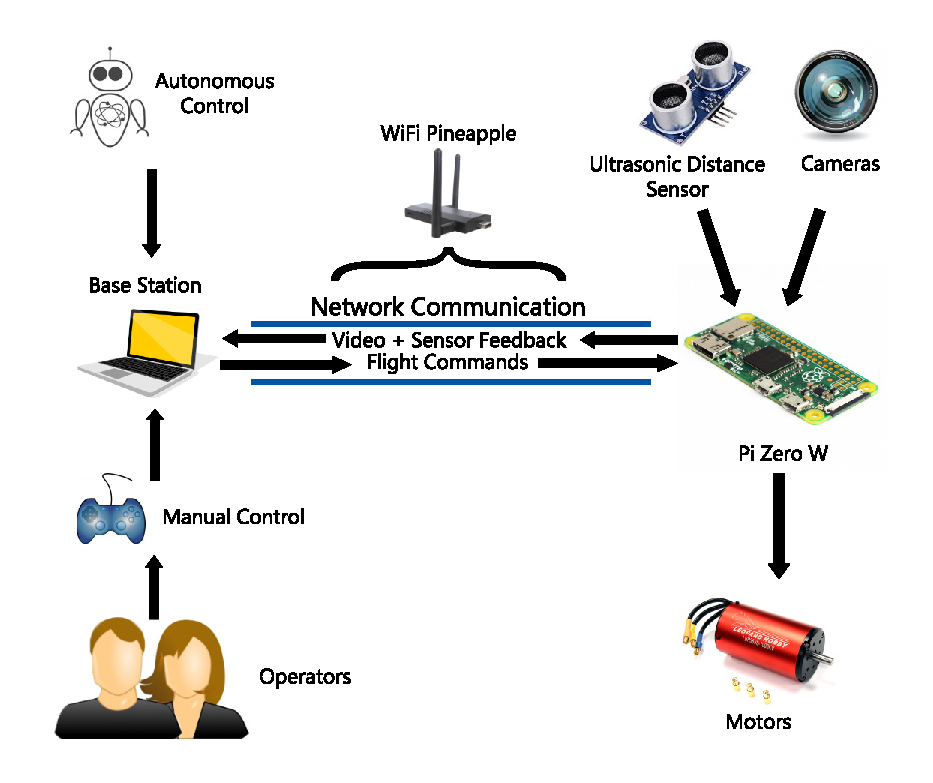
\includegraphics[height=3.5in]{DesignOverview}
\caption{Conceptual Design Overview}
\end{figure}


\subsection{Design Components}

\subsubsection{Device Communication} 

The communication between the aircraft and the base station will be connected by Wi-Fi. Data is transferred over a 2.4GHz channel, allowing Raspberry Pi board and base station to receive and transmit data when they are in the range of a Wi-Fi network. We will establish a Wi-Fi network by using a router, specifically the WiFi Pineapple \cite{r12}. In the event of communication loss, the vehicle should attempt to reconnect for no more than 3 seconds. If the connection is not re-established, the vehicle will shut down the motors. 


\subsubsection{Hardware}

The two main logic control components are the base station and the Raspberry Pi \cite{r3}. These two components will be able to communicate to eachother through the WiFi Pineapple router. The Base station will handle the difficult computations regarding image processing and flight planning. Additionally, the base station will be able to select between manual control mode or autonomous control mode using a GUI. The Raspberry Pi will handle motor control logic, and elevation control. Video and sensor information will be bassed from the Raspberry Pi to the base station, and directional commands will be returned from the base station to the Pi. 


\subsubsection{Flight Control}

We will connect motor controllers to the Raspberry Pi with GPIO pins. We will write a GPIO access program to access GPIO pins and establish communication with motors. We can configure the GPIO pins to start and shutdown the motors. Furthermore, we can set the logical voltages either low or high to change the speed. This code to control the motors will be able to handle commands from both manual and autonomous inputs.


\subsubsection{Sensors}% (camera + ultrasonic)

Camera Sensors are used to easily capture images. For the manual flight, the camera sensor will stream video (image frames) back to the base station. For the autonomous operation, these “images” can be used by video-processing algorithms for recognizing the target, searching the home-base, and operating the hover-hold. We will equip two cameras to our aircraft. One front Camera to process stream video and one at the bottom to find targets and the landing places.


The ultrasonic sensor can emit a specific frequency of sound waves and listen to that sound wave bounce back. The sensor can record the elapsed time between the sound wave being emitted and the sound wave bouncing back. \cite{r11} Once we know the speed of the sound wave, it is able to calculate the distance between the ultrasonic sensor and the object. we will use an ultrasonic sensor at the bottom of aircraft to detect the height from the ground and measure the boundary range.


\subsubsection{Image Processing}

All image processing will be done on the base station to increase calculation performance. Image processing should be able to distinguish four main objects: Delivery targets, packages, boundary lines, and obstacles. Once these objects are correctly identified, the autonomous system will then have to identify where that object is located in correlation to the vehicle. After a general location is established (Left, Right, in front, below, ect.) The autonomous system should then send the appropriate flight commands to the vehicle. 

\subsubsection{User Interface}

The user interface should be simple, with only the necissary information needed to control the micro air vehicle displayed. There should be a white button to enable manual flight control, as well as a red button to stop all flight commands. At minimum the front facing camera stream will be displayed on the user interface. The second camera stream may be added if computational power is not significantly compromised. Additionally, image processing overlays may also be added under the same circumstances. 



\section{Design Viewpoints} % (viewpoints are just an in-depth explanation of a certain aspect of the design)

\subsection{Introduction}  
	Viewpoints are an in-depth evaluation for each of our above design components. Here we will break each viewpoint into three primary categories: design concerns, design elements, and design examples. Design concerns address what we are trying to solve, and what problems we are anticipating to come accross. Design elements will break down the specific goals of each viewpoint. Within the deign elements we will elaborate on each specific task and a general idea of how it will be implemented. In design examples we will review any existing technologies that might solve the viewpoint we are addressing. If there are no exisiting technologies, then we will review similar applications and explaine what we are doing differently. 



\begin{center}
    \begin{tabular}{|c|p{0.3\linewidth}|p{0.4\linewidth}|}
        \hline
		Design viewpoint & Design concerns & Example Design Concepts \\
        \hline
		Communication & Reliability, Fail-safe Operations  & Video streaming applications and standard data packet transfer over WiFi.  \\
		\hline 
        Hardware & Reliable, Lightweight, Multifunctional & Raspberry pi, CSI cameras, Ultrasonic sensors, WiFi Pineapple\\
		\hline 
        Image Processing & Object Detection, Directional Translation & OpenCV \cite{r8}, Matlab Image toolbox \cite{r9}, directional markers  \\
		\hline 
        Flight Control & Motor control, Logic outline, Input Arguments  & ESC motor controller and GPIO pins.  \\
		\hline 
        Positioning & Ultrasonic Distance sensors, Image distance calculations  & OpenCV distance and positioning calculations, distance based on sultrasonic readings.  \\
		\hline 
        User control & User Interface, Manual Control Methods, Emergency Shutdown  &   \\
		\hline 
    \end{tabular}
\end{center}

    

\subsection{Communication Viewpoint} 
\begin{itemize}
 \item{ \textbf{Design Concerns:}}

The main design concern for communication is maintaining a low-latency, high-bandwidth connection between a base station and the vehicle. Design considerations should be made based on what will best address the above design constraint. Additional concerns about communication distance and strength will be secondary considerations for this project. \\ 

\item{ \textbf{Design Elements:}}

There are three objects that rely on steady communicaiton channels: The base station, the vehicle, and the router. The router will act as an intermediary to the base station in order to boost the signal range, and produce a local network that the vehicle can connect to. The base station will connect to the router via USB or ethernet cable, and the vehicle will connect over the 2.4GHz wireless channel. This creates a closed network that we can easily secure to communicate from our base station to our vehicle and back. Video and Ultrasonic Sensor information will be passed from the vehicle to the base station, and the flight calculations will be returned to the vehicle for execution. \\

\item{ \textbf{Design Examples:}}

Typically MAV's are controlled using radio communication, so our approach to this is not conventional. The main reason behind this is because WiFi has limited range compared to radio communication methods. For our applicaiton we will be in relatively close proximity to the vehicle, so this makes WiFi a better option for data throughput. \\


\end{itemize}



\subsection{Hardware Viewpoint} 
\begin{itemize}
\item{ \textbf{Design Concerns:}}

\item{ \textbf{Design Elements:}}

\item{ \textbf{Design Examples:}} %If there are any!

\end{itemize}



\subsection{Image Processing Viewpoint}
\begin{itemize}
\item{ \textbf{Design Concerns:}}

The concerns of the imgage processing can seperate into two parts: object detection and directional translation. In competition, the object is the envelop with two colour which are white and red. The envelop might not in the original video range at the beginning, so the detection depends on the path of microhelicopter. During flighting, the angles of the cameras are changing. Causes by the view of object, the shape of object is also changing. POsition and various of shape can increase the difficulty of object detection. After the detection, the path of pick up package need to be calculate. 
\item{ \textbf{Design Elements:}}

\item{ \textbf{Design Examples:}} %If there are any!

\end{itemize}



\subsection{Flight Control Viewpoint} %(how do we talk to the motors)
\begin{itemize}
\item{ \textbf{Design Concerns:}}

The main design concern for flight control is maintaining a stable connection between the Raspberry Pi with the multiple ESC motor controllers and motors. Additional concerns will be ESC motor controller sending the correct pulsing signals to motors with the command receive from the users. \\

\item{ \textbf{Design Elements:}}

Flight control will be accomplished by firstly connect the ESC motor controllers with the Raspberry Pi through the GPIO pins. Then, we will have each ESC motors controller separately connect with each motor and with an extended power bank. We will write a GPIO access program to access GPIO pins and write output to the ESC motor controllers, then procced the signal to the motors. Once the connection completed, users can control the flight by sending command to the Raspberry Pi board.\\
\item{ \textbf{Design Examples:}} %If there are any!

\end{itemize}



\subsection{Positioning Viewpoint} %(distance + camera positioning)
\begin{itemize}
\item{ \textbf{Design Concerns:}}

\item{ \textbf{Design Elements:}}

\item{ \textbf{Design Examples:}} %If there are any!

\end{itemize}



\subsection{User Control Viewpoint}% (how do we talk to the pi, talk about GUI)
\begin{itemize}
\item{ \textbf{Design Concerns:}}

\item{ \textbf{Design Elements:}}

\item{ \textbf{Design Examples:}} %If there are any!

\end{itemize}


\section{Conclusion}

The Micro Air Vehicle challenge not only encompasses the design requirements listed above, but also the design requirements put forth by the Electrical and Mechanical sub-teams. While this design document provides a comprehensive coverage of the logical systems required, there are additional contributions that are not specified above. This document adequately outlines the design requirements for the Computer Science sub-team attached to Oregon State University's Micro Air Vehicle Challenge team. 


\bibliographystyle{IEEEtran}
\bibliography{references}

\newpage

\section{Timeline}

\vspace{2mm}

\begin{rotate}{270}
\begin{ganttchart}[
    hgrid style/.style={black, dotted},
    vgrid={*5{black,dotted}, *1{white, dotted}, *1{black, dashed}},
    x unit=.8mm,
    y unit chart=9mm,
    y unit title=12mm,
    time slot format=isodate,
    group label font=\bfseries \Large,
    link/.style={->, thick}
    ]{2017-10-04}{2018-06-21}
    \gantttitlecalendar{year, month=name}\\

    \ganttgroup[
        group/.append style={fill=blue}
    ]{Systems Build}{2017-10-04}{2018-5-12}\\ [grid]
	
    \ganttbluebar[
        name=Communications
    ]{Communications}{2017-10-07}{2017-11-12}\\ [grid] 
	
    \ganttbluebar[
    	name=Motor Control
    ]{Motor Control}{2017-11-12}{2018-01-15}\\ [grid]   
	
    \ganttbluebar[
    	name=Flight Control
    ]{Flight Control}{2018-1-11}{2018-02-30}\\ [grid]    
	
    \ganttbluebar[
    	name=User Interface
    ]{User Interface}{2017-12-12}{2018-3-13}\\ [grid]
	
    \ganttbluebar[
    	name=Image Recognition
    ]{Image Recognition}{2017-12-12}{2018-3-13}\\ [grid]

    \ganttbluebar[
    	name=Integration Testing
    ]{Integration Testing}{2018-3-13}{2018-5-12}\\ [grid]

    \ganttgroup[
        group/.append style={fill=orange}
    ]{Competition}{2017-11-9}{2018-05-16}\\ [grid]
	
    \ganttorangebar[
        name=Design proposal
    ]{Design proposal}{2017-11-20}{2018-01-30}\\ [grid]
	
	\ganttorangebar[
        name=Final Selection
    ]{Final Selection}{2018-01-30}{2018-03-17}\\ [grid]
	
	\ganttorangebar[
        name=Event Participation
    ]{Event Participation}{2018-05-12}{2018-05-16}\\ [grid]
    
    \ganttgroup[
        group/.append style={fill=green}
    ]{Expo Preparation}{2018-05-16}{2018-06-15}\\ [grid]
    
\end{ganttchart}
\end{rotate}







\end{document}
